%%
%% This is file `sigconf.tex',
%% generated with the docstrip utility.
%%
%% The original source files were:
%%
%% samples.dtx  (with options: `all,proceedings,sigconf')
%% 
%% IMPORTANT NOTICE:
%% 
%% For the copyright see the source file.
%% 
%% Any modified versions of this file must be renamed
%% with new filenames distinct from sigconf.tex.
%% 
%% For distribution of the original source see the terms
%% for copying and modification in the file samples.dtx.
%% 
%% This generated file may be distributed as long as the
%% original source files, as listed above, are part of the
%% same distribution. (The sources need not necessarily be
%% in the same archive or directory.)
%%
%%
%% Commands for TeXCount
%TC:macro \cite [option:text,text]
%TC:macro \citep [option:text,text]
%TC:macro \citet [option:text,text]
%TC:envir table 0 1
%TC:envir table* 0 1
%TC:envir tabular [ignore] word
%TC:envir displaymath 0 word
%TC:envir math 0 word
%TC:envir comment 0 0
%%
%% The first command in your LaTeX source must be the \documentclass
%% command.
%%
%% For submission and review of your manuscript please change the
%% command to \documentclass[manuscript, screen, review]{acmart}.
%%
%% When submitting camera ready or to TAPS, please change the command
%% to \documentclass[sigconf]{acmart} or whichever template is required
%% for your publication.
%%
%%
\documentclass[11pt,sigconf,nonacm]{acmart}

% Reduce margins
\geometry{
    top=1.0in,
    bottom=1.0in,
    inner=1.0in,
    outer=1.0in,
    footskip=13pt,
    ignoreheadfoot,
    columnsep=14pt,
    heightrounded=false
}

\newcommand{\cacheExt}{\texttt{cache\_ext}}

\usepackage{xcolor}
\usepackage{enumitem}

%%
%% \BibTeX command to typeset BibTeX logo in the docs
\AtBeginDocument{%
  \providecommand\BibTeX{{%
    Bib\TeX}}}

%% Rights management information.  This information is sent to you
%% when you complete the rights form.  These commands have SAMPLE
%% values in them; it is your responsibility as an author to replace
%% the commands and values with those provided to you when you
%% complete the rights form.

%% These commands are for a PROCEEDINGS abstract or paper.

%%
%%  Uncomment \acmBooktitle if the title of the proceedings is different
%%  from ``Proceedings of ...''!
%%
%%\acmBooktitle{Woodstock '18: ACM Symposium on Neural Gaze Detection,
%%  June 03--05, 2018, Woodstock, NY}


%%
%% Submission ID.
%% Use this when submitting an article to a sponsored event. You'll
%% receive a unique submission ID from the organizers
%% of the event, and this ID should be used as the parameter to this command.
%%\acmSubmissionID{123-A56-BU3}

%% (\include{caption} removed: there is no caption.tex and \include forces a page break)

%%
%% For managing citations, it is recommended to use bibliography
%% files in BibTeX format.
%%
%% You can then either use BibTeX with the ACM-Reference-Format style,
%% or BibLaTeX with the acmnumeric or acmauthoryear sytles, that include
%% support for advanced citation of software artefact from the
%% biblatex-software package, also separately available on CTAN.
%%
%% Look at the sample-*-biblatex.tex files for templates showcasing
%% the biblatex styles.
%%
%%
%% The majority of ACM publications use numbered citations and
%% references.  The command \citestyle{authoryear} switches to the
%% "author year" style.
%%
%% If you are preparing content for an event
%% sponsored by ACM SIGGRAPH, you must use the "author year" style of
%% citations and references.
%% Uncommenting
%% the next command will enable that style.
%%\citestyle{acmauthoryear}

%%
%% end of the preamble, start of the body of the document source.
\begin{document}

%%
%% The "title" command has an optional parameter,
%% allowing the author to define a "short title" to be used in page headers.
\title{Optimizing page cache policy for Heterogeneous Storage via \texttt{cache\_ext}}

%%
%% The "author" command and its associated commands are used to define
%% the authors and their affiliations.
%% Of note is the shared affiliation of the first two authors, and the
%% "authornote" and "authornotemark" commands
%% used to denote shared contribution to the research.

\author{Arjun Anil}
\affiliation{
    \institution{University of Wisconsin--Madison}
    \city{Madison}
    \country{USA}
}
\email{aanil3@wisc.edu}

\author{Aidan Liaw}
\affiliation{
    \institution{The University of Queensland}
    \city{Brisbane}
    \country{Australia}
}
\email{aidan.liaw@student.uq.edu.au}

\author{Sayali Kulkarni}
\affiliation{
    \institution{University of Wisconsin--Madison}
    \city{Madison}
    \country{USA}
}
\email{sskulkarni34@wisc.edu}

%%
%% By default, the full list of authors will be used in the page
%% headers. Often, this list is too long, and will overlap
%% other information printed in the page headers. This command allows
%% the author to define a more concise list
%% of authors' names for this purpose.
\renewcommand{\shortauthors}{Anil et al.}

%%
%% The abstract is a short summary of the work to be presented in the
%% article.
\begin{abstract}
  The emergence of \cacheExt has arose a variety of experiments on page cache policies, via it's ability to modify such policies without modifications to the Linux kernel. This has motivated us to re-explore past research into heterogeneous storage caching policies, under modern storage devices, and modern homogeneous cache policies, adapted for heterogeneous storage systems. We see that under [POLICIES] that [RESULTS], and conclude that [CONCLUSION].
\end{abstract}

%%
%% The code below is generated by the tool at http://dl.acm.org/ccs.cfm.
%% Please copy and paste the code instead of the example below.
%%

%%
%% Keywords. The author(s) should pick words that accurately describe
%% the work being presented. Separate the keywords with commas.

%%
%% This command processes the author and affiliation and title
%% information and builds the first part of the formatted document.
\maketitle


% \section{Introduction}


% \section{Experiment}

% \subsection{Variables}


% \subsection{Apparatus}

% \begin{figure}[t]
%     \centering
%     \includegraphics[width=\columnwidth]{latency_throughput.png}
%     \caption{Minimum one-way latency (left axis) and best throughput (right axis) versus transfer size; dotted lines mark \texttt{PIPE\_BUF} and the pipe capacity.}
%     \label{fig:lat-tp}
%     \Description{Latency and throughput against message size on two logarithmic axes.}
% \end{figure}


% Figure~\ref{fig:lat-tp} shows that a small message takes about 1\,$\mu$s one way (0.98\,$\mu$s at 4B), stepping up to 2.12\,$\mu$s at 4KB, and beyond the pipe capacity latency is roughly proportional to the size (113.9\,$\mu$s at 512KB). Throughput rises from 21\,MiB/s (4B) to a peak of 4,742\,MiB/s at 16KB, is 25\% lower at 64KB (3,578\,MiB/s) and stays there up to 512KB. The minima reproduced to within 0.9--9.7\% (latency) and 5.8--14\% (throughput, chunks of 1KB and larger; 29--39\% for 4B and 16B) across five runs.

\providecommand{\tbd}[1]{\textcolor{red}{[#1]}}

\section{Introduction}

% Background summary.

As AI applications drive memory demand and outpace growth in supply, many live storage solutions from DRAM down to HDDs have increased in price from 2026 onwards \cite{memory_prices}. This has caused adopting a prudent outlook for RAM usage both in terms of \textit{percentage used} and \textit{pages resident}.

This price rise has motivated data centres to increase the deployment of SSDs and HDDs \cite{tcostorage, ssdhddmarket}, and ongoing research into best optimising their combined usage \cite{tcostorage, declarativeio, heterogeneousssd}. Recent research has sought to use heterogeneous storage for cost optimisation and dataset placement \cite{tcostorage}, reduce redundant storage I/O 

% Current policy work.

Specific to page cache policy, such research begun with Forney et al. \cite{Forney}, which identified that "storage-aware" cache policies demonstrate performance benefits via simulating ageing (varying performance) HDDs. Research on HDD and SSD storage configurations can be traced to Kim et al. \cite{ssdhddfirst}, that simulates both the replacement policy and the heterogeneous storage. 

On the matter of cache policies, the emergence of [POLICY INTRODUCTION].

% Motivation.

However, confirmed (via OA journals) research on page caching policies for heterogeneous storage has not been performed since 2012 \cite{lastpaper}, in which both SSDs and HDDS have changed, motivating a revisit to the problem under modern paging policy research and modern storage devices. Under the initial literature review, no paper has yet been discovered that has implemented a homogeneous storage page cache policy on bare metal.

Simultaneously, the introduction of \cacheExt by Zussman et al. has introduced a non-intrusive approach towards modifying Linux's cache policy. \\ \texttt{cache\_ext} is a patched Linux kernel (v6.6.8) that enables custom page cache eviction and admission policies via extended Berkley Package Filter (eBPF) hooks and functions. Critically, it enables per-application policies and a wide variety of data structures to contain pages, enabling targeted testing.

% Challenges.

Thus, We propose the hypothesis: \textbf{To what extent can heterogeneous SSD and HDD storage-aware page cache eviction policies improve performance, and what are the policies that correspond to benefits or impedance to specific workloads?}

Additionally, we predict that: \textbf{A page cache policy that treats files from two different \textit{types} of disks will not be able to optimise for performance gaps. It is "cheaper", latency-wise, to fault in a page from a faster disk compared to a slower one.}

% This problem has become widespread to the point where discussions of an "IO wall" for HDDs (the cheapest of the live secondary storage solutions) has now motivated research into optimising HDD storage \cite{declarativeio}.

% Simultaneously, SSD solutions have trended to lower performance solutions. By increasing the amount of state a given NAND cell stores, progressing from single-level cell (SLC, holding \(2^1 = 2\) states) NAND up to proposed penta-level cell (PLC, holding \(2^5 = 32\) states) NAND, newer NAND solutions enable higher density storage, but sacrifice performance (a key characteristic of SSDs over HDDs) and critically write endurance \cite{qlc}.

\section{Background and Motivation}

\subsection{Heterogeneous Storage}

In the context of heterogeneous storage, this discussion concerns the combination of SSDs and HDDs, which will be briefly summarised.

HDDs in general have a lower cost per unit of storage capacity due to their lower manufacturing cost, whereas SSDs have lower access latencies and higher I/O throughput, especially for random accesses whereby the burden of mechanical movement is nonexistent \cite{arch, tcostorage}. However, in addition to higher costs at lower capacities, they suffer from write endurance (and depending on the technology read endurance too) \cite{arch, tcostorage, heterogeneousssd}. 

Additionally, these properties are not fixed for a device class. Wu et al.\cite{orthus} show that on modern devices the storage \textit{hierarchy} is not strict: device performance can overlap and under load a saturated faster device can serve requests more slowly than the device beneath it. The cost of reading a page is therefore a function of both the device and it's current load, not of the device type alone.

From a page caching perspective however, this heterogeneity means that the cost of both page admission and eviction is dependent on the backing storage device \cite{forney, arch}.

\subsection{Linux Page Caching}

To clarify, the term page and folio are used

\subsection{Motivation}

Software solutions have largely assumed that all storage behaves alike. The Linux page cache, the main layer that hides storage latency from applications. evicts pages by recency and frequency alone, treating every page as equally costly to lose \cite{multigenlru}. On a host with both an SSD and an HDD, re-reading an evicted HDD page takes roughly 50-100 times longer than an SSD page \cite{ssdvshdd}. The kernel thus minimises the number of misses rather than time applications spend waiting on them, and on mixed-device hosts it routinely trades a cheap SSD miss for an expensive HDD one.

This idea is not new: Forney et. al ~\cite{forney} proposed storage-aware caching in 2002, but evaluated it only in simulation, and Meta's TMO~\cite{tmo} showed that reclaim decisions depends on the backing device's performance. Revisting this question in the era of NVMe and Optane devices, Wu et al.\cite{orthus} argue that the storage hierarchy is no longer a hierarchy and that caching layers which assume the cache device is always faster leave substantial performance unused, by upto $2\times$. Additionally, research on heterogeneous storage solutions, have demonstrated that mixed SSD and SSD + HDD solutions may yield higher performance metrics. For example, Takai et al. \cite{heterogeneousssd} have demonstrated that SSD cell type mixtures can enable higher IOPS/cost under specific workloads.

% One existing software solution is \texttt{cache\_ext}, a patched v6.6.8 Linux kernel that enables page caching customisation via the extended Berkley Packet Filter (eBPF) \cite{cacheext}. Its main benefit is that it enables cache policy customisation without Linux kernel code modification.

An existing customisability solution for the Linux page cache is \texttt{cache\_ext}, a patched v6.6.8 kernel \cite{cacheext}. It enables page cache policy customisation without kernel code modification via the extended Berkley Packet Filter (eBPF) interface. We aim to use eBPF to show how a cache policy accommodating heterogeneity might be beneficial for performance.

% This motivates us to merge these two ideas to recreate the performance benefits of existing heterogeneous storage solutions with the flexibility of eBPF.

\subsection{Background on Storage Technologies}

% SSDs

% HDDs

\subsection{Current Linux Page Eviction Policies}

MGLRU

S3-FIFO

LRU with active, inactive list approximation

\subsection{\cacheExt}

\subsection{Related Works}

Apple's Fusion Drive offerings from 2012 to 2019

Intel Optane Memory

\textbf{Non-hierarchical caching.} The closest modern work to ours is Orthus\cite{orthus}, which, like Forney at al.\ \cite{forney} questions the assumption that caching layers sit in a strict performance hierarchy. Orthus introduces \textit{non-hierarchical caching} (NHC) for a fast storage device that caches a slower one. A feedback controller tunes two knobs: it stops admitting data into the cache once the cache already holds the hot set, and it redirects a fraction of hits on clean data to the capacity device so that both devices' bandwidth is used. It is implemented as a block-layer caching module (Orthus-CAS) and as a key-value store cache (Orthus-KV), and improves performance by up to $2\times$ over classic caching.

\tbd{Candidate for cutting if space is not there}. Our setting differs in three ways. First, the page cache is in DRAM and both the SSD and the HDD are backing stores. Orthus caches between two storage devices. Second, our devices hold disjoint data: there are no redundant copies between the SSD and the HDD, so Orthus' central mechanism of redirecting hits to the other device does not apply. Third, the performance gap between a SATA SSD and an HDD is roughly two orders of magnitude, so the inversion that Orthus exploits, where the faster device becomes the bottle, is unlikely on our hardware setup. We therefore act on a different decision policy i.e \textit{which page to evict}, but share Orthus' principle that the right decision depends on device cost rather than on an assumed ordering of devices.

\subsection{Hypothesis and Prediction}



\section{Design}

\subsection{Design Objectives}

% Policies here
\subsection{Proposed policies}
% \subsection{Storage-Awareness Integration}
% \subsection{Predicted Trade-Offs}
% Better if these headsing are coalesced together

Talk about the following for each:
- Policy arch
- How is the storage-awareness part included
- Predicted trade-offs


\section{Implementation}

\texttt{cache\_ext} is a patched Linux kernel (v6.6.8), so we need root access and the ability to boot a custom kernel on a machine with both an SSD and an HDD, most likely using the bootloader \texttt{grub}.

\begin{itemize}[
    leftmargin=2.0em,
    labelsep=0.3em,
    topsep=1pt,
    itemsep=0pt,
    parsep=0pt
]
    \item \textbf{Hardware:} CloudLab Wisconsin bare-metal nodes, which pair HDDs with an SSD in one machine. 
    \item \textbf{Software:} the \texttt{cache\_ext} kernel and sample policies, clang/libbpf/bpftool, cgroup-v2 for limiting memory and reading I/O pressure. 
    % [NEED TO DECIDE ON THE WORKLOADS] -> mentioned in the proposed evaluation methodology section.
\end{itemize}

 
\section{Experimental Setup and Methodology}
\label{sec:setup}
 
\subsection{Testbed}
 
We use a CloudLab bare-metal node with 2 CPU cores and 2\,GB of RAM, running the \cacheExt{} kernel (Linux 6.6.8). A node with both an SSD and an HDD was not available in time for these experiments, so we emulate a slower device. A single physical disk is split into two partitions, each formatted with ext4. The first is used directly as the \emph{fast} device. The second is placed behind Linux's \texttt{dm-delay} device-mapper target, configured with a 5\,ms delay on reads and writes, and serves as the \emph{slow} device. Because \texttt{dm-delay} works in kernel timer ticks, the effective delay differs from the configured value, so we report measured latencies: under our synthetic workload, reads that reached the disk took 18\,ms on average on the fast device and 29\,ms on the slow device, a ratio of about 1.6. Both partitions share one physical disk, which we believe to be a hard drive. \tbd{Arjun: confirm the disk model and the node type, and add the second node (SSD + HDD) once results from it are available.}
 
\subsection{Workloads}
 
\subsubsection{Synthetic Two-Device Microbenchmark}
 
We use fio~\cite{fio} with eight threads issuing 4\,KB random reads through the page cache (\texttt{psync}, buffered I/O). The workload reads two 512\,MB files, one on each device. Each read chooses one of the two files uniformly at random, so both files receive the same number of requests, and chooses an offset within that file from a Zipfian distribution with $\theta = 0.9$. All threads share a single hot set. Each thread issues its next read only when the previous one completes. The workload therefore models a single application that depends equally on data stored on two devices of different speeds, and it isolates one variable: the two files are equally popular, so any difference in how a policy treats them comes from the device they are stored on.
 
\subsubsection{Production Block I/O Traces}
 
To evaluate policies on realistic access patterns, we will replay two public production traces:
 
\begin{itemize}[leftmargin=1.5em, topsep=2pt, itemsep=1pt]
    \item \textbf{Meta Tectonic (Baleen)}~\cite{baleen}. Anonymised requests from Meta's production bulk storage system (Tectonic), recorded at a CacheLib flash cache placed in front of it. Seven traces are provided, each sampled by block ID from a different storage cluster, and each request records a block ID, byte offset, I/O size, timestamp and operation. Down-sampled versions (0.1\% and 1\%) are provided, each intended to be used with a cache of the same relative size.
    \item \textbf{Alibaba Cloud block traces}~\cite{alibabatraces}. All I/O to 1{,}000 virtual disks, randomly sampled from a production elastic block storage cluster, over January 2020. Each record contains a disk ID, read/write flag, byte offset, length and timestamp. The full trace is 181\,GB compressed and 751\,GB uncompressed, so we will use a subset of disks and a time window.
\end{itemize}
 
\textbf{Replay.} We will convert the read requests of each trace into fio's I/O log format and replay them with fio through the page cache (buffered I/O) in a single cgroup, so that the same harness, memory limits and metrics apply as for the synthetic workload. Each trace volume (a Tectonic block or an Alibaba virtual disk) is mapped to a file, and the files are placed on the fast and slow devices. \tbd{Decide: (a) how volumes are assigned to devices, e.g.\ randomly, by access frequency (hot data on the fast or the slow device), or by size; (b) whether to replay writes; (c) whether to replay at the recorded timestamps or as fast as possible; (d) which subset and time window to use, and how offsets are scaled to fit the node's disk and memory.} Because both traces were recorded below a cache in the original system (the Baleen traces at a flash cache in front of HDDs, the Alibaba traces at the block device of each virtual disk, below the guest's page cache), part of the original reuse has already been absorbed upstream; we expect lower hit rates than with the synthetic workload and will report them.
 
\subsection{Memory Limit}
 
Each workload runs in one cgroup v2 whose \texttt{memory.max} limits its page cache, with swap disabled. For the synthetic workload we use 64, 128 and 256\,MB, between one sixteenth and one quarter of the 1\,GB of data, so the policy must continually choose which pages to evict. \tbd{Memory limits for the trace replays, chosen relative to each trace's footprint.} Because a \cacheExt{} policy is attached per cgroup, the pages of both devices are managed by the same policy.
 
\subsection{Procedure}
 
For each policy and memory limit we:
\begin{enumerate}[leftmargin=1.5em, topsep=2pt, itemsep=1pt]
    \item drop the page cache;
    \item create the cgroup and, for \cacheExt{} policies, load the policy;
    \item fill the cache by reading \texttt{memory.max} worth of data with sequential 1\,MB reads, alternating 8\,MB chunks between the two files, so that the cache is full and eviction begins immediately without favouring either file;
    \item run the workload for 240\,s without measuring, so that the cache contents reflect the policy rather than the initial fill (at the measured rate of about 340 misses per second, this replaces even the 256\,MB cache at least once);
    \item run the workload for 30\,s and measure.
\end{enumerate}
The cgroup's name must begin with \texttt{cache\_ext}: the \cacheExt{} kernel enables the policy hooks only for such cgroups. In any other cgroup the policy's \texttt{init} hook runs but its page-level hooks are never called, and the kernel's default policy evicts all pages. We verify every policy run by enabling BPF run-time statistics and checking that the run counts of \texttt{folio\_added}, \texttt{folio\_accessed} and \texttt{evict\_folios} increase during the run. We report one run per configuration. \tbd{Increase to at least three runs per configuration for the final report.}
 
\subsection{Metrics}
 
From fio we record throughput (IOPS) and tail latency (p99). From \texttt{/proc/diskstats} we record, for each device, the number of reads that reached the device (page cache misses) and the time spent on them, from which we compute the average read latency. After each run we record the fraction of each file resident in the page cache using \texttt{mincore}. Cache hits are computed as fio reads minus device reads.
 
We check each run for validity: the cgroup was 86--97\% full at the start of measurement, so eviction was taking place; every device read transferred exactly 4\,KB, so read-ahead did not bring in additional pages; and the node was otherwise idle, since \texttt{/proc/diskstats} counts I/O from all processes.
 
\subsection{Policies}
 
We compare the default kernel policy (classic two-list LRU, with MGLRU disabled), MGLRU, and the two-list biased LRU (one LRU list per device; each eviction request is served from the fast device's list with probability 0.75, falling back to the other list if needed). As a check that \cacheExt{} policies take effect on our testbed, we also ran the \cacheExt{} MRU policy at 64\,MB, with a 120\,s warm-up. \tbd{Add the cost-aware policy once implemented.}
 
\section{Evaluation}
\label{sec:eval}
 
\begin{figure*}[t]
    \centering
    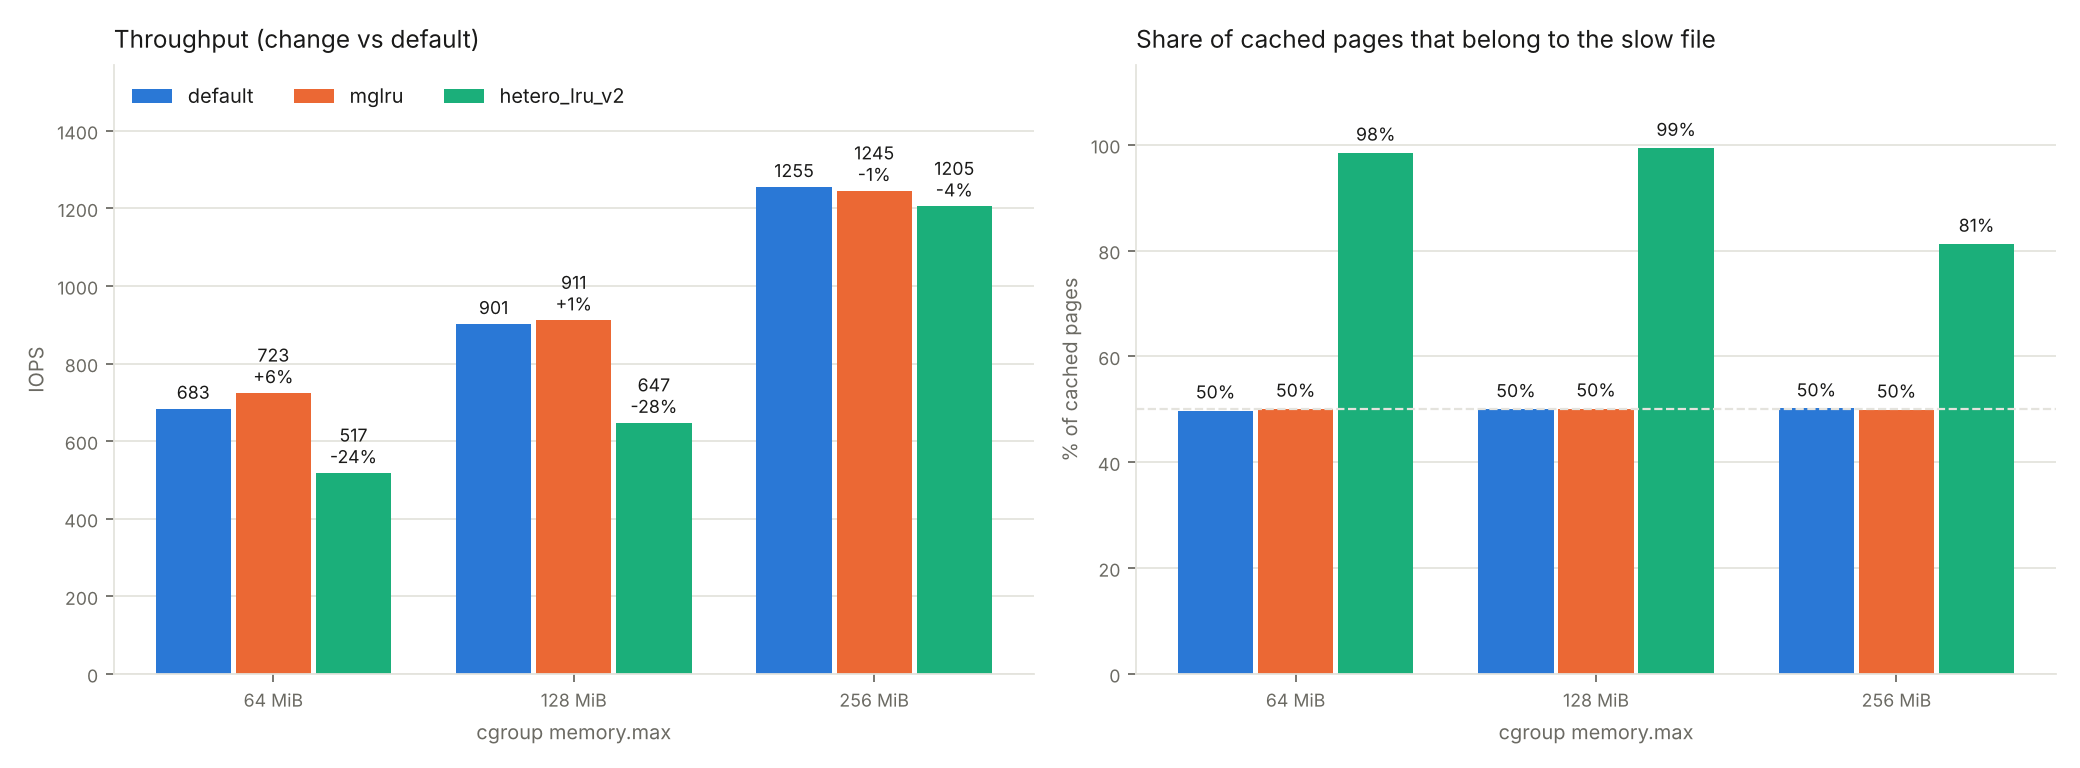
\includegraphics[width=\textwidth]{hetero_fio_policies.png}
    \caption{Synthetic workload. Left: throughput of each policy, with the change relative to the default policy. Right: share of cached pages that belong to the slow device's file at the end of each run.}
    \label{fig:policies}
    \Description{Two grouped bar charts over memory limits of 64, 128 and 256 MB. Left: IOPS for default, MGLRU and the two-list LRU; the two-list LRU is 24 and 28 percent lower at 64 and 128 MB and 4 percent lower at 256 MB. Right: default and MGLRU hold 50 percent slow-file pages; the two-list LRU holds 98, 99 and 81 percent.}
\end{figure*}
 
\begin{table}[t]
  \centering
  \small
  \setlength{\tabcolsep}{4pt}
  \begin{tabular}{rrrrr}
    \toprule
    Limit & Default & MGLRU & Two-list & Slow \\
    \midrule
    64\,MB  & 683  & 723 (+6\%)  & 517 ($-$24\%)  & 98\% \\
    128\,MB & 901  & 911 (+1\%)  & 647 ($-$28\%)  & 99\% \\
    256\,MB & 1255 & 1245 ($-$1\%) & 1205 ($-$4\%) & 81\% \\
    \bottomrule
  \end{tabular}
  \caption{Synthetic workload: throughput (IOPS) by policy and cgroup memory limit. \emph{Slow} is the share of cached pages belonging to the slow file under the two-list LRU (50\% for the default and MGLRU).}
  \label{tab:results}
\end{table}
 
\subsection{Existing Policies Ignore the Device}
 
Under both the default policy and MGLRU, the two files are cached equally at every memory limit (3.6\%, 8.8\% and 21.5\% of each file at 64, 128 and 256\,MB for the default policy), and the two devices see almost the same number of misses (about 5{,}100 each in 30\,s). The two policies also perform almost identically: MGLRU is within 6\% of the default at every size (Table~\ref{tab:results}). Throughput rises with the memory limit, from 683 to 1255 IOPS for the default policy, as the hit rate rises from 50\% to 73\%.
 
Because a miss on the slow device costs about 1.6 times as much as a miss on the fast device, this even split is not even in cost. With the default policy, the slow device accounts for 61--62\% of the total disk read time while receiving half of the misses.
 
\subsection{A Fixed Bias Reduces Throughput}
 
The two-list LRU changes how the cache is divided as intended: the slow file's pages make up 98\%, 99\% and 81\% of the cached pages at 64, 128 and 256\,MB (Figure~\ref{fig:policies}, right), and reads that reach the disk shift from an even split to roughly two fast-device reads for every slow-device read. However, throughput falls by 24\% and 28\% at 64 and 128\,MB and by 4\% at 256\,MB (Figure~\ref{fig:policies}, left), and p99 latency rises from 64--68\,ms to 82--87\,ms at the two smaller sizes.
 
The cause is lost hits. At 64\,MB the fast file keeps only about 0.4\,MB (about 100 pages) in the cache, compared with 18\,MB under the default policy, even though it receives half of all reads. Hits in 30\,s fall from 10{,}273 to 4{,}749 (a hit rate of 31\% instead of 50\%), while the number of misses barely changes (10{,}247 versus 10{,}786). At 128\,MB hits fall from 16{,}928 to 8{,}030. The policy evicts the fast file's most frequently used pages in order to keep slow-file pages that are used less often, because the biased coin chooses which list to evict from regardless of how recently the pages in that list were used. When the fast list holds only about a hundred pages, its least recently used page was typically accessed moments earlier.
 
The disk is saturated in every configuration: it completes about 340--380 misses per second regardless of the policy, and the eight threads spend almost all of their time waiting on it, so the fast and slow read times add up to about 240\,s per 30\,s run (eight threads $\times$ 30\,s) under every policy. In this regime throughput is determined by the hit rate, and a policy that reduces hits reduces throughput even if it moves misses to the faster device. With 256\,MB of cache, the fast file keeps 8\% of its pages resident and the loss shrinks to 4\%.
 
Sharing one disk also affects per-device latency: under the two-list LRU, reads on the fast device became faster (13--15\,ms) and reads on the slow device slower (36--43\,ms), as the mix of requests at the disk changed.
 
\subsection{Sanity Check}
 
The \cacheExt{} MRU policy, which evicts the most recently used pages, achieves 365 IOPS at 64\,MB compared with 683 for the default, and its hooks were invoked tens of thousands of times during the run, confirming that \cacheExt{} policies control eviction on our testbed. Runs made in a cgroup without the \texttt{cache\_ext} prefix matched the default policy exactly and are excluded.
 
\subsection{Trace-Driven Evaluation}
 
\tbd{Results of replaying the Baleen and Alibaba traces (Section~\ref{sec:setup}): throughput, hit rate and per-device misses for each policy and memory limit. Not yet run.}
 
\subsection{Summary}
 
On the synthetic workload, the default policy and MGLRU divide the cache evenly between the fast and slow devices, so the slow device dominates disk read time. A fixed bias towards keeping slow-device pages corrects the division but discards frequently used fast-device pages and lowers throughput by up to 28\%. These results are from an emulated slow device only about 1.6 times slower than the fast one, with both on the same disk; with a real SSD and HDD, the benefit of keeping slow-device pages should be much larger.
 


\section{Discussion}

\subsubsection{Implications}

\subsubsection{Limitations}

\subsubsection{Related Works}

\subsubsection{Future Work}

\textbf{Load-adaptive cost.} Orthus \cite{orthus} uses a feedback driven design to adapt to dynamically changing loads. We can measure per-device miss latency in eBPF from the block-layer tracepoints and use it to update the parameter the policy uses (like the break-even-interval ratio for the five-minute rule policy). 

\section{Conclusion}

\section{Acknowledgements}


% Additionally, with different mediums of secondary storage available, from Hard Disk Drives (HDDs) to Solid State Drives (SSDs) to Storage Attached Networks (SANs), has caused the . 

It is also worth noting performance disparities in a \textit{class} of secondary storage. For example, SSD solutions have trended to lower performance solutions via increasing the state stored by NAND cells, moving from single-level cell up to proposed penta-level cell. These newer cell solutions enable higher density storage, but sacrifice performance and write endurance \cite{qlc}.

We would like to point out that heterogeneous storage solutions differ from tiered storage solutions. Heterogeneous solutions can be defined as appearing as a single storage mechanism, and how this mechanism performs. By contrast, tiered solutions can be defined as a policy on data placement.

Considering the heterogeneous nature of secondary storage, in performance, a page cache policy that treats files from two different \textit{types} of disks will not be able to optimise for performance gaps. It is "cheaper", latency-wise, to fault in a page from a faster disk compared to a slower one.

% \section{Evaluation and Methodology}

% Until prices stabilise or fall, new solutions in secondary storage are needed to provide equivalent performance on lower performance devices to keep costs down. This however, requires new software solutions to form.

% Software solutions have largely assumed that all storage behaves alike. The Linux page cache, the main layer that hides storage latency from applications. evicts pages by recency and frequency alone, treating every page as equally costly to lose \cite{multigenlru}. On a host with both an SSD and an HDD, re-reading an evicted HDD page takes roughly 50-100 times longer than an SSD page \cite{ssdvshdd}. The kernel thus minimises the number of misses rather than time applications spend waiting on them, and on mixed-device hosts it routinely trades a cheap SSD miss for an expensive HDD one.

% This idea is not new: Forney et. al ~\cite{forney} proposed storage-aware caching in 2002, but evaluated it only in simulation, and Meta's TMO~\cite{tmo} showed that reclaim decisions depends on the backing device's performance. Additionally, research on heterogeneous storage solutions, have demonstrated that mixed SSD and SSD + HDD solutions may yield higher performance metrics. For example, Takai et al. \cite{heterogeneousssd} have demonstrated that SSD cell type mixtures can enable higher IOPS/cost under specific workloads.

% One existing software solution is \texttt{cache\_ext}, a patched v6.6.8 Linux kernel that enables page caching customisation via the extended Berkley Packet Filter (eBPF) \cite{cacheext}. Its main benefit is that it enables cache policy customisation without Linux kernel code modification.

% An existing customisability solution for the Linux page cache is \texttt{cache\_ext}, a patched v6.6.8 kernel \cite{cacheext}. It enables page cache policy customisation without kernel code modification via the extended Berkley Packet Filter (eBPF) interface. We aim to use eBPF to show how a cache policy accommodating heterogeneity might be beneficial for performance.

% This motivates us to merge these two ideas to recreate the performance benefits of existing heterogeneous storage solutions with the flexibility of eBPF.

% \section{Criticisms and Next Steps}

% Our plan involves the following:

% \begin{enumerate}[label=(\arabic*), leftmargin=2.0em, labelsep=0.3em]
    % \item \textbf{Setup and Baselines.} Build and boot a kernel with \texttt{cache\_ext}, and reproduce its baseline policies (default LRU, MGLRU, and the sample policies provided by the authors) to validate our environment.

    % \item \textbf{Heterogeneous storage testbed.} Configure a system with at least two storage devices of differing performance, for example a fast NVMe SSD and a slower QLC device. If real QLC hardware is unavailable, we will emulate the slower device by adding latency or throttling bandwidth through a \texttt{shim}.

    % \item \textbf{Heterogeneous storage testbed.} Configure a system with at least two storage devices of differing performance. If real hardware is unavailable, we will emulate the slower device by adding latency or throttling bandwidth through a \texttt{shim}.


    % \item \textbf{Storage-aware eviction policy.} Implement an eBPF policy in \texttt{cache\_ext} that tracks cached page to devices and weighs eviction decisions by the cost of a future miss on that device. We will start by exploring Forney et al.'s partition-based approach which divides the cache per device and resizes partitions to balance the work across devices, and compare it against a simpler cost-weighted variant of LRU.

% \end{enumerate}

% \section{Proposed Evaluation Methodology}

% We will be comparing our policy against the baselines on file-system microbenchmarks (fio) and application workloads such as key-value store. We will measure throughput, tail latency, per-device miss counts, and the amount of DRAM needed to reach a target level of performance, which ties the results back to the cost argument behind TMO.

% The exact workload characteristics needs to be pinned down by literature review (for example, whether the GET-SCAN workload that \texttt{cache\_ext} uses be an option).

% \section{Resources Required}

% \texttt{cache\_ext} is a patched Linux kernel (v6.6.8), so we need root access and the ability to boot a custom kernel on a machine with both an SSD and an HDD, most likely using the bootloader \texttt{grub}.

% \begin{itemize}[
%     leftmargin=2.0em,
%     labelsep=0.3em,
%     topsep=1pt,
%     itemsep=0pt,
%     parsep=0pt
% ]
%     \item \textbf{Hardware:} CloudLab Wisconsin bare-metal nodes, which pair HDDs with an SSD in one machine. 
%     \item \textbf{Software:} the \texttt{cache\_ext} kernel and sample policies, clang/libbpf/bpftool, cgroup-v2 for limiting memory and reading I/O pressure. 
%     % [NEED TO DECIDE ON THE WORKLOADS] -> mentioned in the proposed evaluation methodology section.
% \end{itemize}

% \section{AI Usage}

% It is our plan to involve AI in our project. We will use AI for the implementation of our proposed policy. Our AI usage will follow closely with the AI policy of CS736. Critically, we will not use AI for idea generation, \textcolor{blue}{\href{https://dictionary.cambridge.org/us/dictionary/english/waffling}{writing}} (except making LaTeX .bib citations) or presentation creation.


\section{Overleaf link}
For reference, our LaTeX source can be found below.
\newline
% \textcolor{blue}{\url{https://www.overleaf.com/read/nrhbnrgdhdzh#16effe}}

\bibliographystyle{ACM-Reference-Format}
\bibliography{sample-base}

\end{document}
\endinput
